\chapter{Kiến thức nền tảng}

\section{Học tăng cường (Reinforcement Learning)}
\subsection{Giới thiệu}
Học tăng cường (Reinforcement Learning) \cite{reinforcementlearninganintroduction} là học cách ánh xạ các tình huống thành hành động để cực đại phần thưởng. Người học không được cho biết hành động nào cần thực hiện, nhưng thay vào đó phải khám phá ra hành động nào mang lại nhiều phần thưởng nhất bằng cách thử chúng. Trong những trường hợp thú vị và khó khăn nhất, các hành động có thể không chỉ ảnh hưởng đến phần thưởng mà còn ảnh hưởng đến tình huống tiếp theo và thông qua đó, cũng ảnh hưởng đến tất cả các phần thưởng tiếp theo. Hai đặc điểm này — tìm kiếm thử-và-sửa sai (trial-and-error) và trì hoãn phần thưởng — là hai đặc điểm phân biệt quan trọng nhất của học tăng cường.

\subsection{Các thành phần của học tăng cường}
Ngoài \textit{agent} (tác nhân) và \textit{environment} (môi trường), người ta có thể xác định bốn thành phần chính của hệ thống học tăng cường: \textit{policy} (chính sách), \textit{reward signal} (tín hiệu phần thưởng), \textit{value function} (hàm giá trị), và có thể có thêm \textit{model} (mô hình) của môi trường.

\begin{itemize}
    \item \textbf{Policy:} xác định cách hoạt động của tác nhân tại một thời điểm nhất định. Nói một cách đại khái, một \textit{policy} là một ánh xạ từ các trạng thái nhận thức của môi trường đến các hành động sẽ được thực hiện khi ở trong các trạng thái đó. Nó tương ứng với những gì trong tâm lý học sẽ được gọi là một tập hợp các quy tắc hoặc liên kết kích thích-phản ứng. Trong một số trường hợp, \textit{policy} có thể là một hàm hoặc bảng tra cứu đơn giản, trong khi trong những trường hợp khác, \textit{policy} có thể liên quan đến tính toán mở rộng chẳng hạn như quá trình tìm kiếm. \textit{Policy} là cốt lõi của một tác nhân học tăng cường theo nghĩa là chỉ nó là đủ để xác định hành vi. Nói chung, các \textit{policy} có thể ngẫu nhiên, chỉ rõ xác suất cho mỗi hành động.
    \item \textbf{Reward signal:} xác định mục tiêu trong vấn đề học tăng cường. Trên mỗi bước thời gian, môi trường gửi cho tác nhân một số duy nhất được gọi là phần thưởng. Mục tiêu duy nhất của tác nhân là tối đa hóa tổng phần thưởng mà tác nhân nhận được trong thời gian dài. Do đó, \textit{reward signal} xác định đâu là những sự kiện tốt và xấu đối với tác nhân. Trong một hệ thống sinh học, chúng ta có thể nghĩ về phần thưởng tương tự như trải nghiệm của niềm vui hoặc nỗi đau. Chúng là các đặc điểm tức thời và xác định vấn đề mà tác nhân phải đối mặt. \textit{Reward signal} là cơ sở chính để thay đổi \textit{policy}; nếu một hành động được \textit{policy} chọn theo sau là \textit{reward} thấp, thì \textit{policy} có thể được thay đổi để chọn một số hành động khác trong tình huống đó trong tương lai. Nói chung, các \textit{reward signal} có thể là các hàm ngẫu nhiên của trạng thái môi trường và các hành động được thực hiện.
    \item \textbf{Value function:} Trong khi \textit{reward signal} cho biết điều gì tốt theo nghĩa tức thời, thì một \textit{value function} chỉ định điều gì tốt về lâu dài. Nói một cách đại khái, \textit{value} của một trạng thái là tổng số phần thưởng mà một tác nhân có thể mong đợi tích lũy trong tương lai, bắt đầu từ trạng thái đó. Trong khi \textit{reward} xác định mong muốn ngay lập tức, nội tại của các trạng thái môi trường, thì các \textit{value} cho thấy mong muốn lâu dài của các trạng thái sau khi tính đến các trạng thái có khả năng tuân theo và \textit{reward} có sẵn trong các trạng thái đó. Ví dụ: một trạng thái có thể luôn mang lại \textit{reward} tức thì thấp nhưng vẫn có \textit{value} cao vì nó thường xuyên được theo sau bởi các trạng thái khác mang lại \textit{reward} cao. Hoặc điều ngược lại có thể đúng. Để so sánh giữa con người với con người, \textit{reward} có phần giống như niềm vui (nếu cao) và nỗi đau (nếu thấp), trong khi \textit{value} tương ứng với sự đánh giá tinh tế hơn và có tầm nhìn xa hơn về mức độ hài lòng hoặc không hài lòng của chúng ta khi môi trường của chúng ta đang ở trong một trạng thái cụ thể.
    \item \textbf{Model environment:} Đây là thứ bắt chước hành vi của môi trường, hay nói chung hơn, cho phép đưa ra các suy luận về cách môi trường sẽ hoạt động. Ví dụ: với một trạng thái và hành động, mô hình có thể dự đoán trạng thái kết quả tiếp theo và phần thưởng tiếp theo. Mô hình được sử dụng để lập kế hoạch, theo đó chúng ta có thể quyết định một quá trình hành động bằng cách xem xét các tình huống có thể xảy ra trong tương lai trước khi chúng thực sự trải qua.
\end{itemize}

\subsection{Ứng dụng của học tăng cường}
Do tính chất của việc học tăng cường là luôn tối ưu việc đạt được phần thưởng cuối cùng dựa vào trạng thái, và phần thưởng hiện tại, cùng với sự tác động của môi trường nên việc học tăng cường được áp dụng nhiều trong các lĩnh vực mang đậm tính tương tác lâu dài giữa tác nhân và môi trường, có thể kể đến:

\begin{itemize}
    \item Điều khiển xe tự hành, robot, v.v.
    \item Các hệ thống gợi ý (Recommendation System), hỏi đáp (Chatbot), v.v.
    \item Ngành công nghiệp trò chơi (game) như là cờ vây (nổi tiếng với AlphaGo), v.v.
\end{itemize}

Cụ thể, trong luận án này sẽ sử dụng phương pháp học tăng cường cho việc huấn luyện mô hình tư vấn khách hàng.

\section{Hệ thống Chatbot hướng mục tiêu (Goal Oriented Chatbot)}
\subsection{Chatbot hướng mục tiêu}
\label{subsec:chatbotgo}
Yêu cầu của một hệ thống tư vấn khách hàng là ta phải đặt cho nó một ngữ cảnh (tư vấn cái gì) và mục tiêu cuối cùng cần hoàn thành khi tư vấn. Vì vậy, đây là một bài toán hướng mục tiêu.

Một Chatbot hướng mục tiêu (GO) cố gắng giải quyết một vấn đề cụ thể cho người dùng. Các Chatbot này có thể giúp mọi người đặt vé, tìm đặt chỗ, v.v. Có hai cách chính để huấn luyện một Chatbot GO: Học có giám sát (supervised learning) với bộ mã hóa-giải mã (encoder-decoder), ánh xạ trực tiếp cuộc đối thoại của người dùng tới phản hồi và học tăng cường giúp huấn luyện một Chatbot thông qua các cuộc hội thoại thử-và-sửa sai (trial-and-error) với người dùng thực hoặc trình mô phỏng người dùng có quy tắc.

Như đã nói từ phần trước, luận án này sử dụng mô hình học tăng cường vì các tối đa lợi thế của nó.

\subsection{Kiến trúc tổng quát của hệ thống Chatbot GO}
Hệ thống đối thoại cho một Chatbot GO sử dụng phương pháp học tăng cường được chia thành 3 phần chính, được mô tả như hình \ref{fig:chatbot}: Phần Quản lý hội thoại (Dialogue Manager), phần Hiểu ngôn ngữ tự nhiên (Natural Language Understanding) và phần Trình tạo ngôn ngữ tự nhiên (Natural Language Generator). Phần Quản lý hội thoại được chia thành Bộ theo dõi trạng thái hội thoại (Dialogue State Tracker) và \textit{policy} cho chính tác nhân, được đại diện bởi mạng nơ-ron (neural network) trong nhiều trường hợp. Ngoài ra, vòng lặp hệ thống chứa một người dùng với các mục tiêu. Mục tiêu người dùng thể hiện những gì người dùng muốn để thoát khỏi cuộc trò chuyện.

\begin{center}
    \begin{figure}[h!]
        \begin{center}
         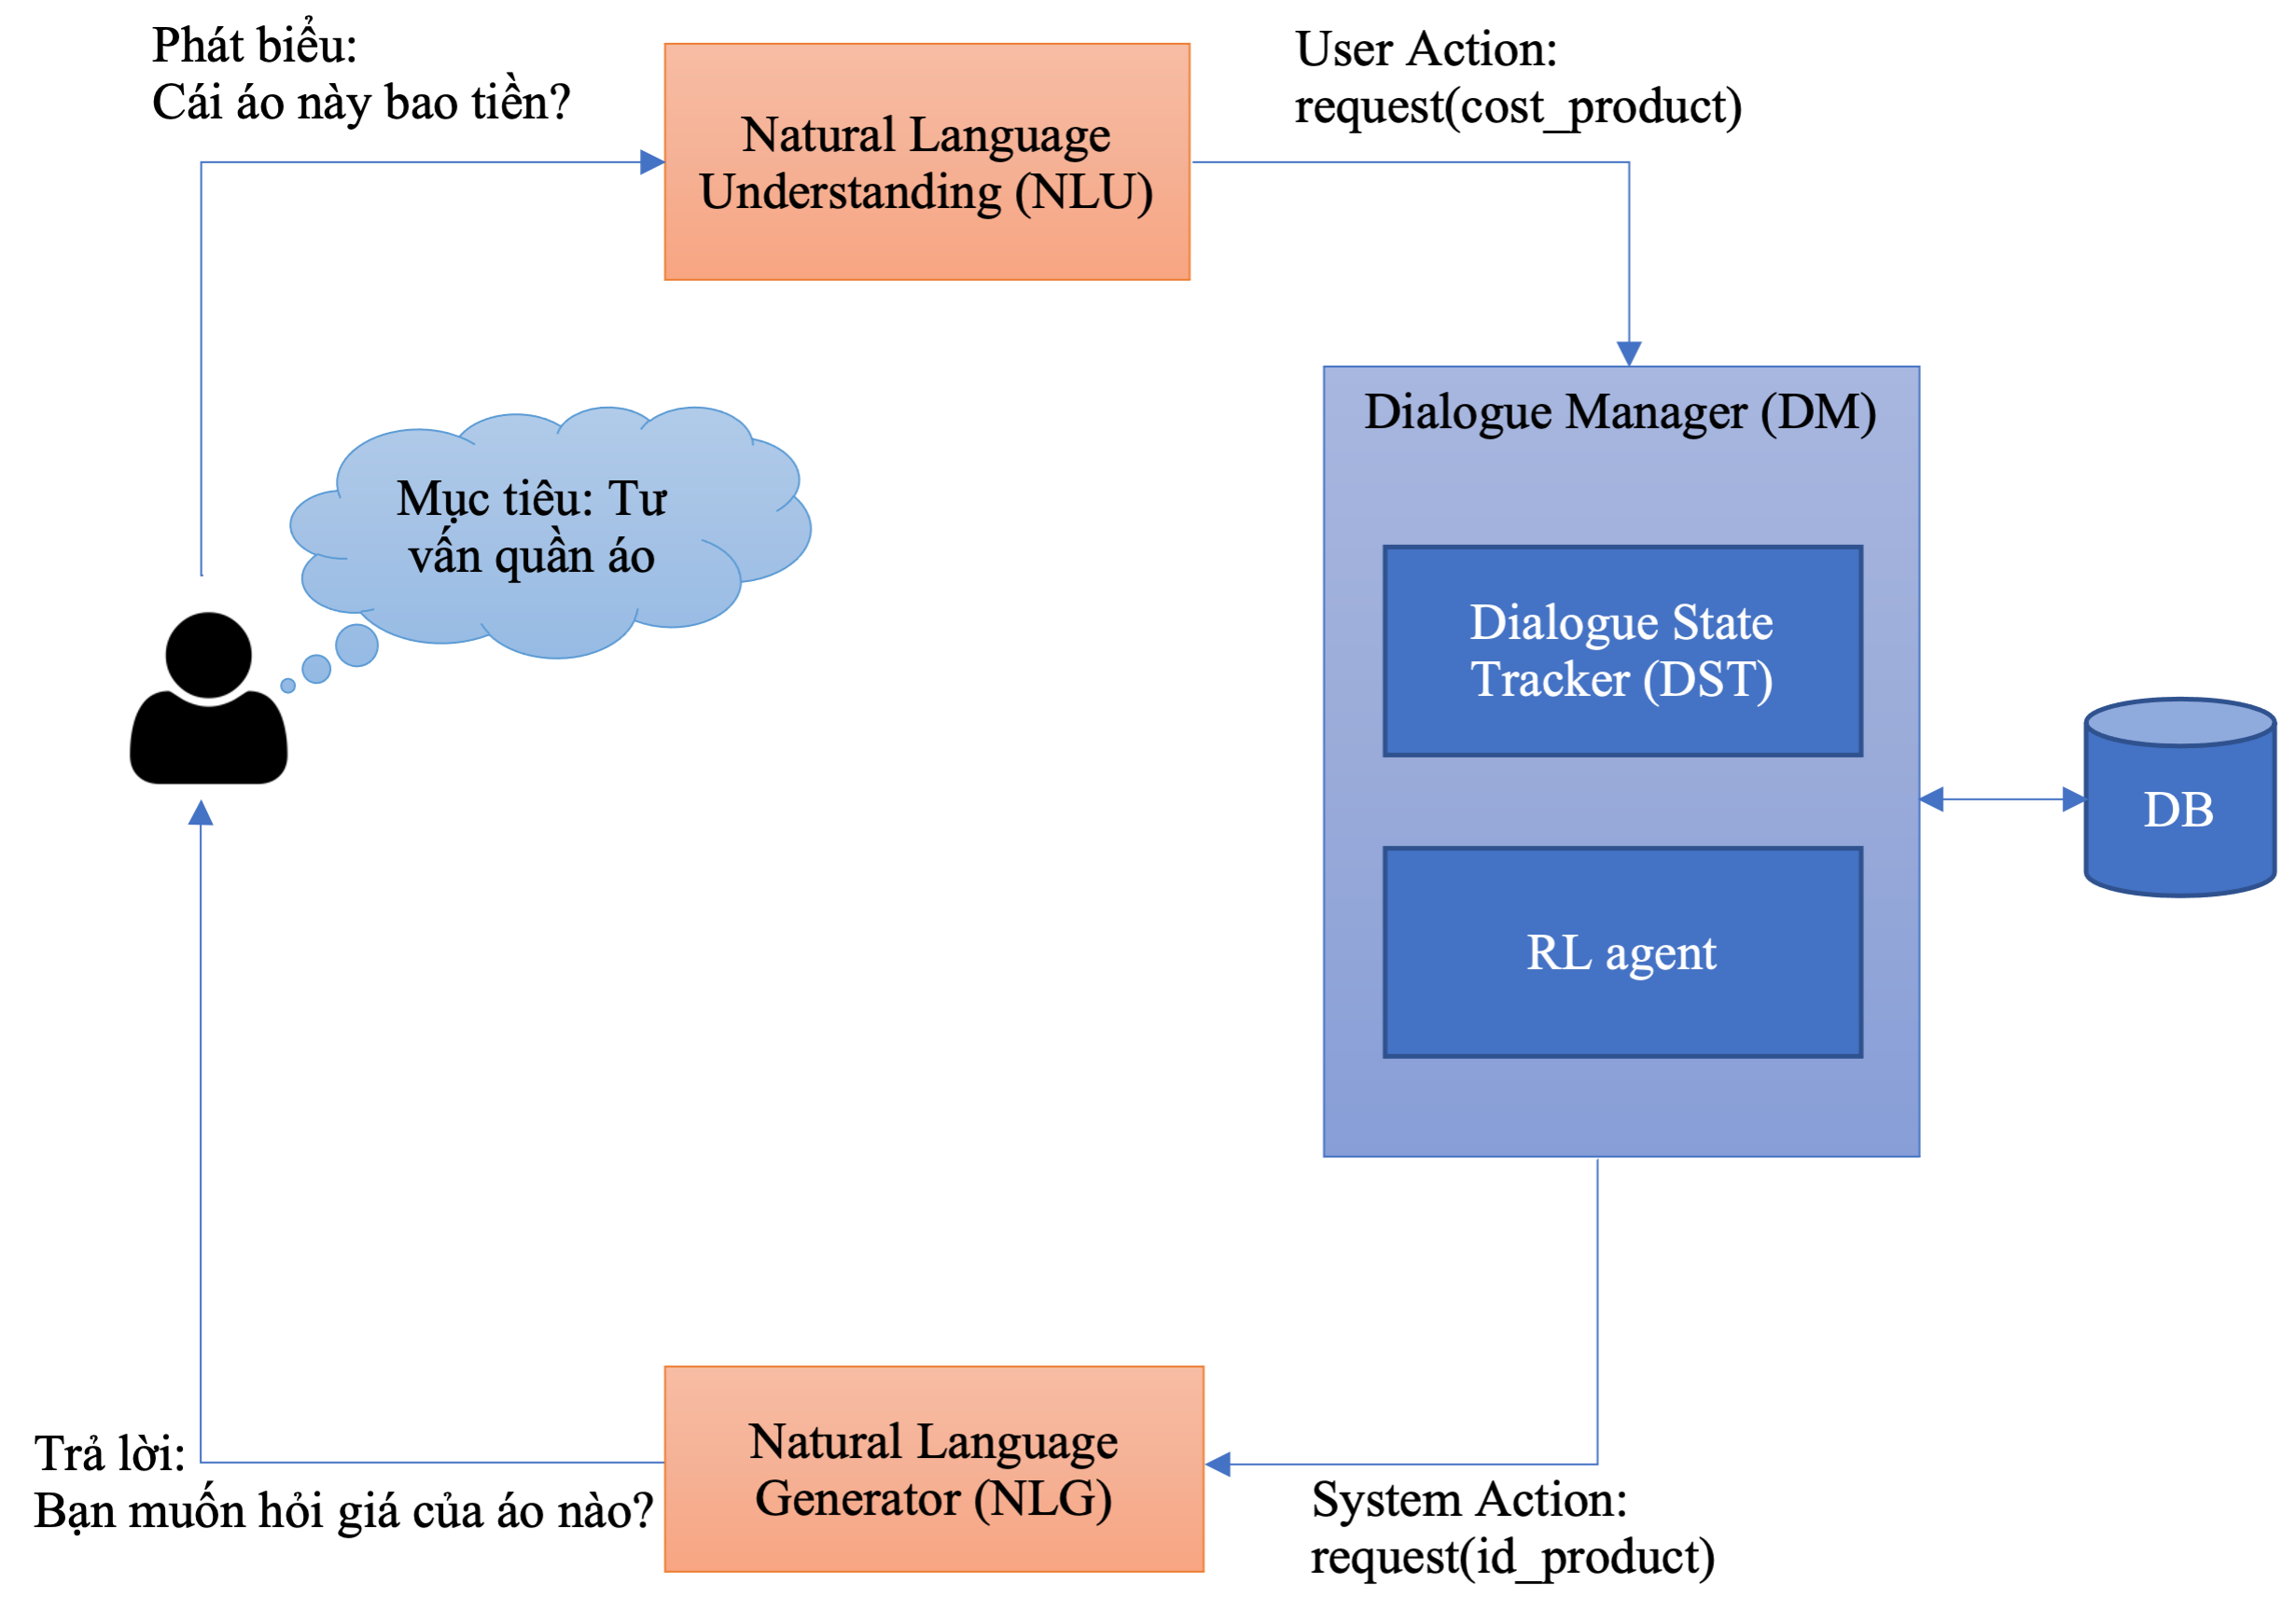
\includegraphics[scale=0.8]{chapter3/img/overviewchatbot.png}
        \end{center}
        \caption{Kiến trúc tổng quát của mô hình Chatbot GO sử dụng phương pháp học tăng cường}
        \label{fig:chatbot}
    \end{figure}
\end{center}

Khi người dùng gửi đi một thông điệp (Cái áo này bao tiền?), sẽ được xử lý bởi thành phần Hiểu ngôn ngữ tự nhiên (NLU), chuyển ngôn ngữ tự nhiên thành một dạng mà tác nhân có thể xử lý, đầu ra (output) là ở dạng khung ngữ nghĩa (semantic frame) (request(cost\_product)).

Sau đó, Bộ theo dõi trạng thái đối thoại (DST) từ hành động của người dùng (đã được chuyển thành khung ngữ nghĩa) và lịch sử của cuộc trò chuyện hiện tại sẽ xử lý và chuyển thành một biểu diễn trạng thái mà có thể xử lý được bởi \textit{policy} của tác nhân. Trạng thái này là đầu vào của \textit{policy} hoặc mạng nơ ron của tác nhân, đầu ra là hành động của tác nhân dưới dạng khung ngữ nghĩa (request(id\_product)).

Cơ sở dữ liệu được truy vấn để thêm thông tin vào cho tác nhân như thông tin các kích thước, màu sắc v.v.

Hành động của tác nhân sau đó được xử lý bởi phần Trình tạo ngôn ngữ tự nhiên (NLG), chuyển nó sang ngôn ngữ tự nhiên để người dùng có thể dễ dàng đọc hiểu (Bạn muốn hỏi giá của áo nào?).

\section{Mô hình học tăng cường cho Chatbot GO}
\label{sec:model}
Như đã đề cập ở mục giới hạn của đề tài \ref{sec:scope}, chúng ta sẽ quan tâm sử dụng mô hình học tăng cường như thế nào để áp dụng vào bài toán hướng mục tiêu tư vấn khách hàng. Trình bày ở mục \ref{subsec:chatbotgo}, một tác nhân Chatbot hướng mục tiêu (GO) sẽ được huấn luyện để trò chuyện thành thạo với người dùng thực nhằm hoàn thành mục tiêu, phù hợp với các ràng buộc của người dùng. Quá trình tác nhân học tập theo phương pháp học tăng cường được mô tả rõ hơn ở hình \ref{fig:learningflow}.

\begin{center}
    \begin{figure}[h!]
        \begin{center}
         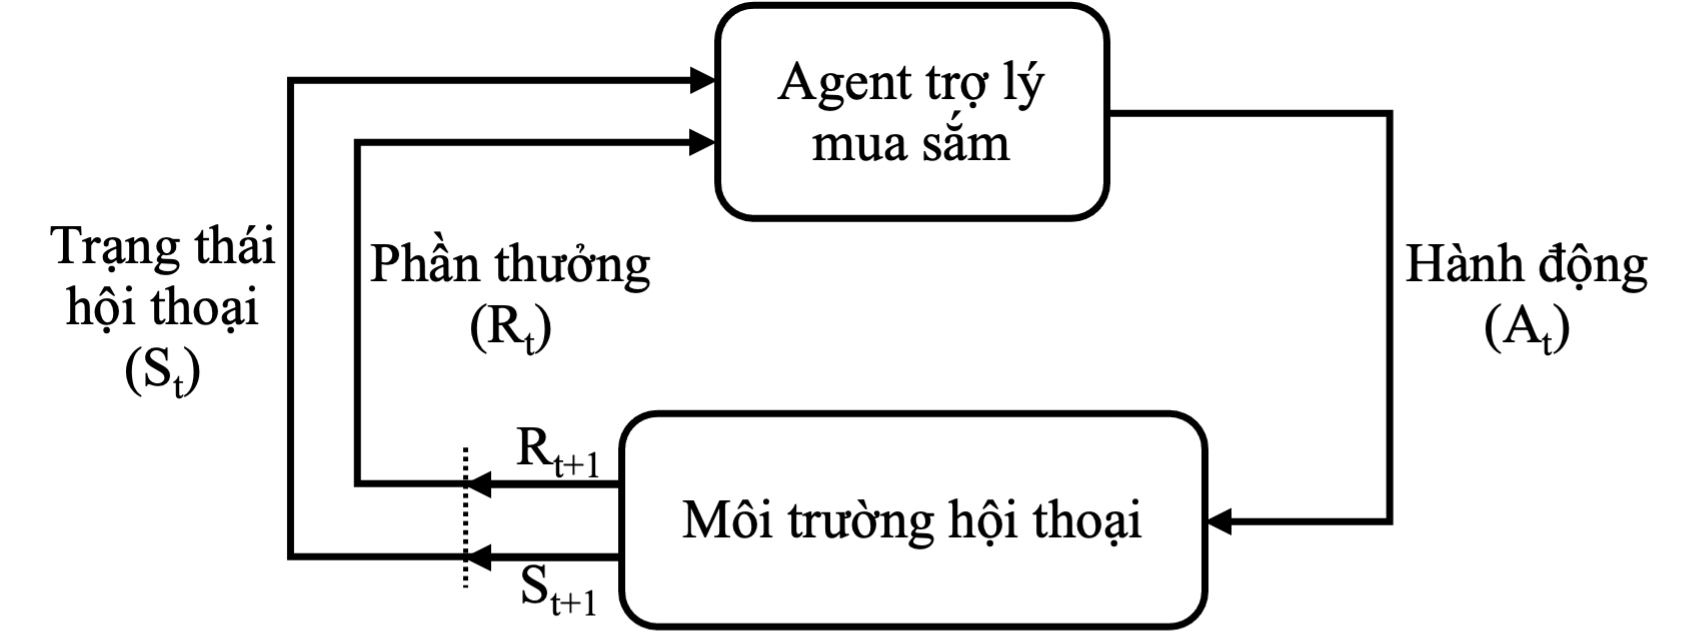
\includegraphics[scale=1]{chapter3/img/learningflow.png}
        \end{center}
        \caption{Quá trình huấn luyện theo phương pháp học tăng cường}
        \label{fig:learningflow}
    \end{figure}
\end{center}

Bản chất của học tăng cường là thử và sửa sai, nó sẽ thử đi thử lại các hành động và rút ra kinh nghiệm sau mỗi lần thử. Trong bài toán tư vấn khách hàng, việc thử này sẽ được thực hiện như sau:

\begin{itemize}
    \item Tại trạng thái hiện tại là $S_t$, tác nhân ngẫu nhiên hoặc theo một luật (policy) nào đó có sẵn chọn ra một hành động $A_t$.
    \item Hành động này sẽ tác động vào môi trường là diễn biến của hội thoại hiện tại cho ra trạng thái mới là $S_{t+1}$ và nhận giá trị là phần thường $R_t$ cho hành động đó.
    \item Phần thưởng này sẽ đánh giá được việc chọn hành động đó có tốt hay không. Từ đó tác nhân cập nhật lại cách chọn hành động.
\end{itemize}

Với mô hình này, ta dễ thấy tác nhân sẽ chỉ nhận đầu vào là trạng thái hội thoại hiện tại để ra quyết định hành động. Vì vậy, ta cần xem xét đến các thông tin cần có trong trạng thái như thế nào để tác nhân có đủ thông tin để ra quyết định. Việc này được trình bày rõ hơn trong mục \ref{subsec:state}.

Trong thời gian đầu, tác nhân có thể ngẫu nhiên chọn các hành động hoặc theo một luật định sẵn đơn giản. Sau đó, nó cần được chỉ ra hành động nào là không tốt, để cập nhập cách chọn hành động (policy), cách thức thực hiện là thông qua điểm thưởng. Các điểm thưởng sẽ được định nghĩa sao cho giống với các yêu cầu của người dùng thật để quá trình tự học của tác nhân là hiệu quả và thỏa mãn với nhu cầu người dùng. Cụ thể được mô tả trong mục \ref{subsec:reward}.

\subsection{Trạng thái hội thoại}
\label{subsec:state}
Trạng thái hội thoại chứa những thông tin hữu ích từ lịch sử hội thoại cho tới thời điểm hiện tại. Các thông tin này có thể khác nhau tùy vào mục đích sử dụng tác nhân. Tuy nhiên, nó nên chứa các thông tin biểu thị tình trạng, những diễn biến đã, đang diễn ra trong hội thoại. Dưới đây diễn giải một số thông tin trong trạng thái hội thoại cho tác nhân trợ lý mua sắm.

Giả sử, ta có một cuộc hội thoại giữa người dùng và cửa hàng diễn ra như sau:

\renewcommand{\lstlistingname}{Ví dụ}
\begin{lstlisting}[caption={Một mẫu đoạn hội thoại},label={exam:dialog1},language=exam_vn,firstnumber=1]
User: Hi shop
Admin: Chào bạn, bạn cần shop tư vấn sản phẩm nào ạ?
User: Chân váy hoa có size gì vậy bạn
Admin: Dạ chân váy hoa bên em có size M, và L ạ
User: Còn màu hồng ko?
Admin: Dạ sản phẩm còn 2 cái ạ
User: OK shop. Mình lấy cái này nha.
Admin: Bạn mặc size gì ạ?
\end{lstlisting}

Tại dòng 3, người dùng hỏi kích thước của sản phẩm. Để tác nhân có thể thực hiện được hành vi đúng là cung cấp thông tin thì nó cần biết rằng yêu cầu hiện tại của người dùng là gì (yêu cầu thông tin kích thước) và thông tin người dùng cung cấp (tên sản phẩm). Vì vậy, trạng thái hội thoại cần chứa hành động hiện tại của người dùng.

Tại dòng 5, người dùng yêu cầu thông tin số lượng và cung cấp thông tin màu sắc. Tuy nhiên, ta biết rằng để tìm kiếm đúng sản phẩm phù hợp, cần biết tên của sản phẩm. Mà tên sản phẩm đã được người dùng cung cấp tại dòng 3. Vì vậy, ngoài hành động hiện tại, trạng thái hội thoại còn chứa tất cả các thông tin mà người dùng đã thông báo trước đó.

Tại dòng 7, người dùng muốn đặt đơn hàng. Để chốt được đơn hàng, cửa hàng cần biết đầy đủ thông tin cần thiết của sản phẩm để tìm thấy một mẫu sản phẩm duy nhất. Như ví dụ trên, chân váy hoa có 2 loại kích cỡ khác nhau. Tác nhân cần yêu cầu người dùng cung cấp thêm thông tin này. Vì vậy trong trạng thái hội thoại cần có kết quả sau khi truy vấn cơ sở dữ liệu của từng thông tin.

Ngoài ra, ta cần có thêm hành động gần nhất của tác nhân để tránh việc lặp lại hành động từ tác nhân. Trong nhu cầu thực tế, việc tư vấn và giúp người dùng đạt mục tiêu cuối cùng nên diễn ra nhanh nhất có thể. Vì vậy, số lượt hội thoại đã diễn ra cũng được thêm vào.

\subsection{Phần thưởng và ảnh hưởng của nó đến quyết định hành động}
\label{subsec:reward}
Ta cần định nghĩa phần thưởng phù hợp cho hành động của tác nhân trong mỗi trạng thái hội thoại khác nhau. Xét ví dụ \ref{exam:dialog1}, ta có thể định nghĩa một số điểm thưởng dựa trên phản hồi của người dùng như sau:

\begin{itemize}
    \item Tại dòng 2, hành động của tác nhân đơn giản là chào hỏi lại người dùng. Hành động này thông thường và phản hồi của người dùng là tiếp nối cuộc trò chuyện. Vì vậy, hành động này có thể xem là hành động qua lượt, không mang giá trị điểm thưởng.
    \item Tại dòng 4, tác nhân cung cấp thông tin mà người dùng yêu cầu từ câu trước, hành động này không bị từ chối bởi người dùng ở câu sau. Vì vậy, hành động này xem là cung cấp giá trị có ích cho người dùng và được 1 điểm thưởng.
\end{itemize}

Sau khi có điểm thưởng cho từng hành động, việc tác nhân cập nhật cách chọn hành động và đưa ra hành động mới như thế nào, ta xét ví dụ sau như hình \ref{fig:dialog2}.

\begin{center}
    \begin{figure}[h!]
        \begin{center}
         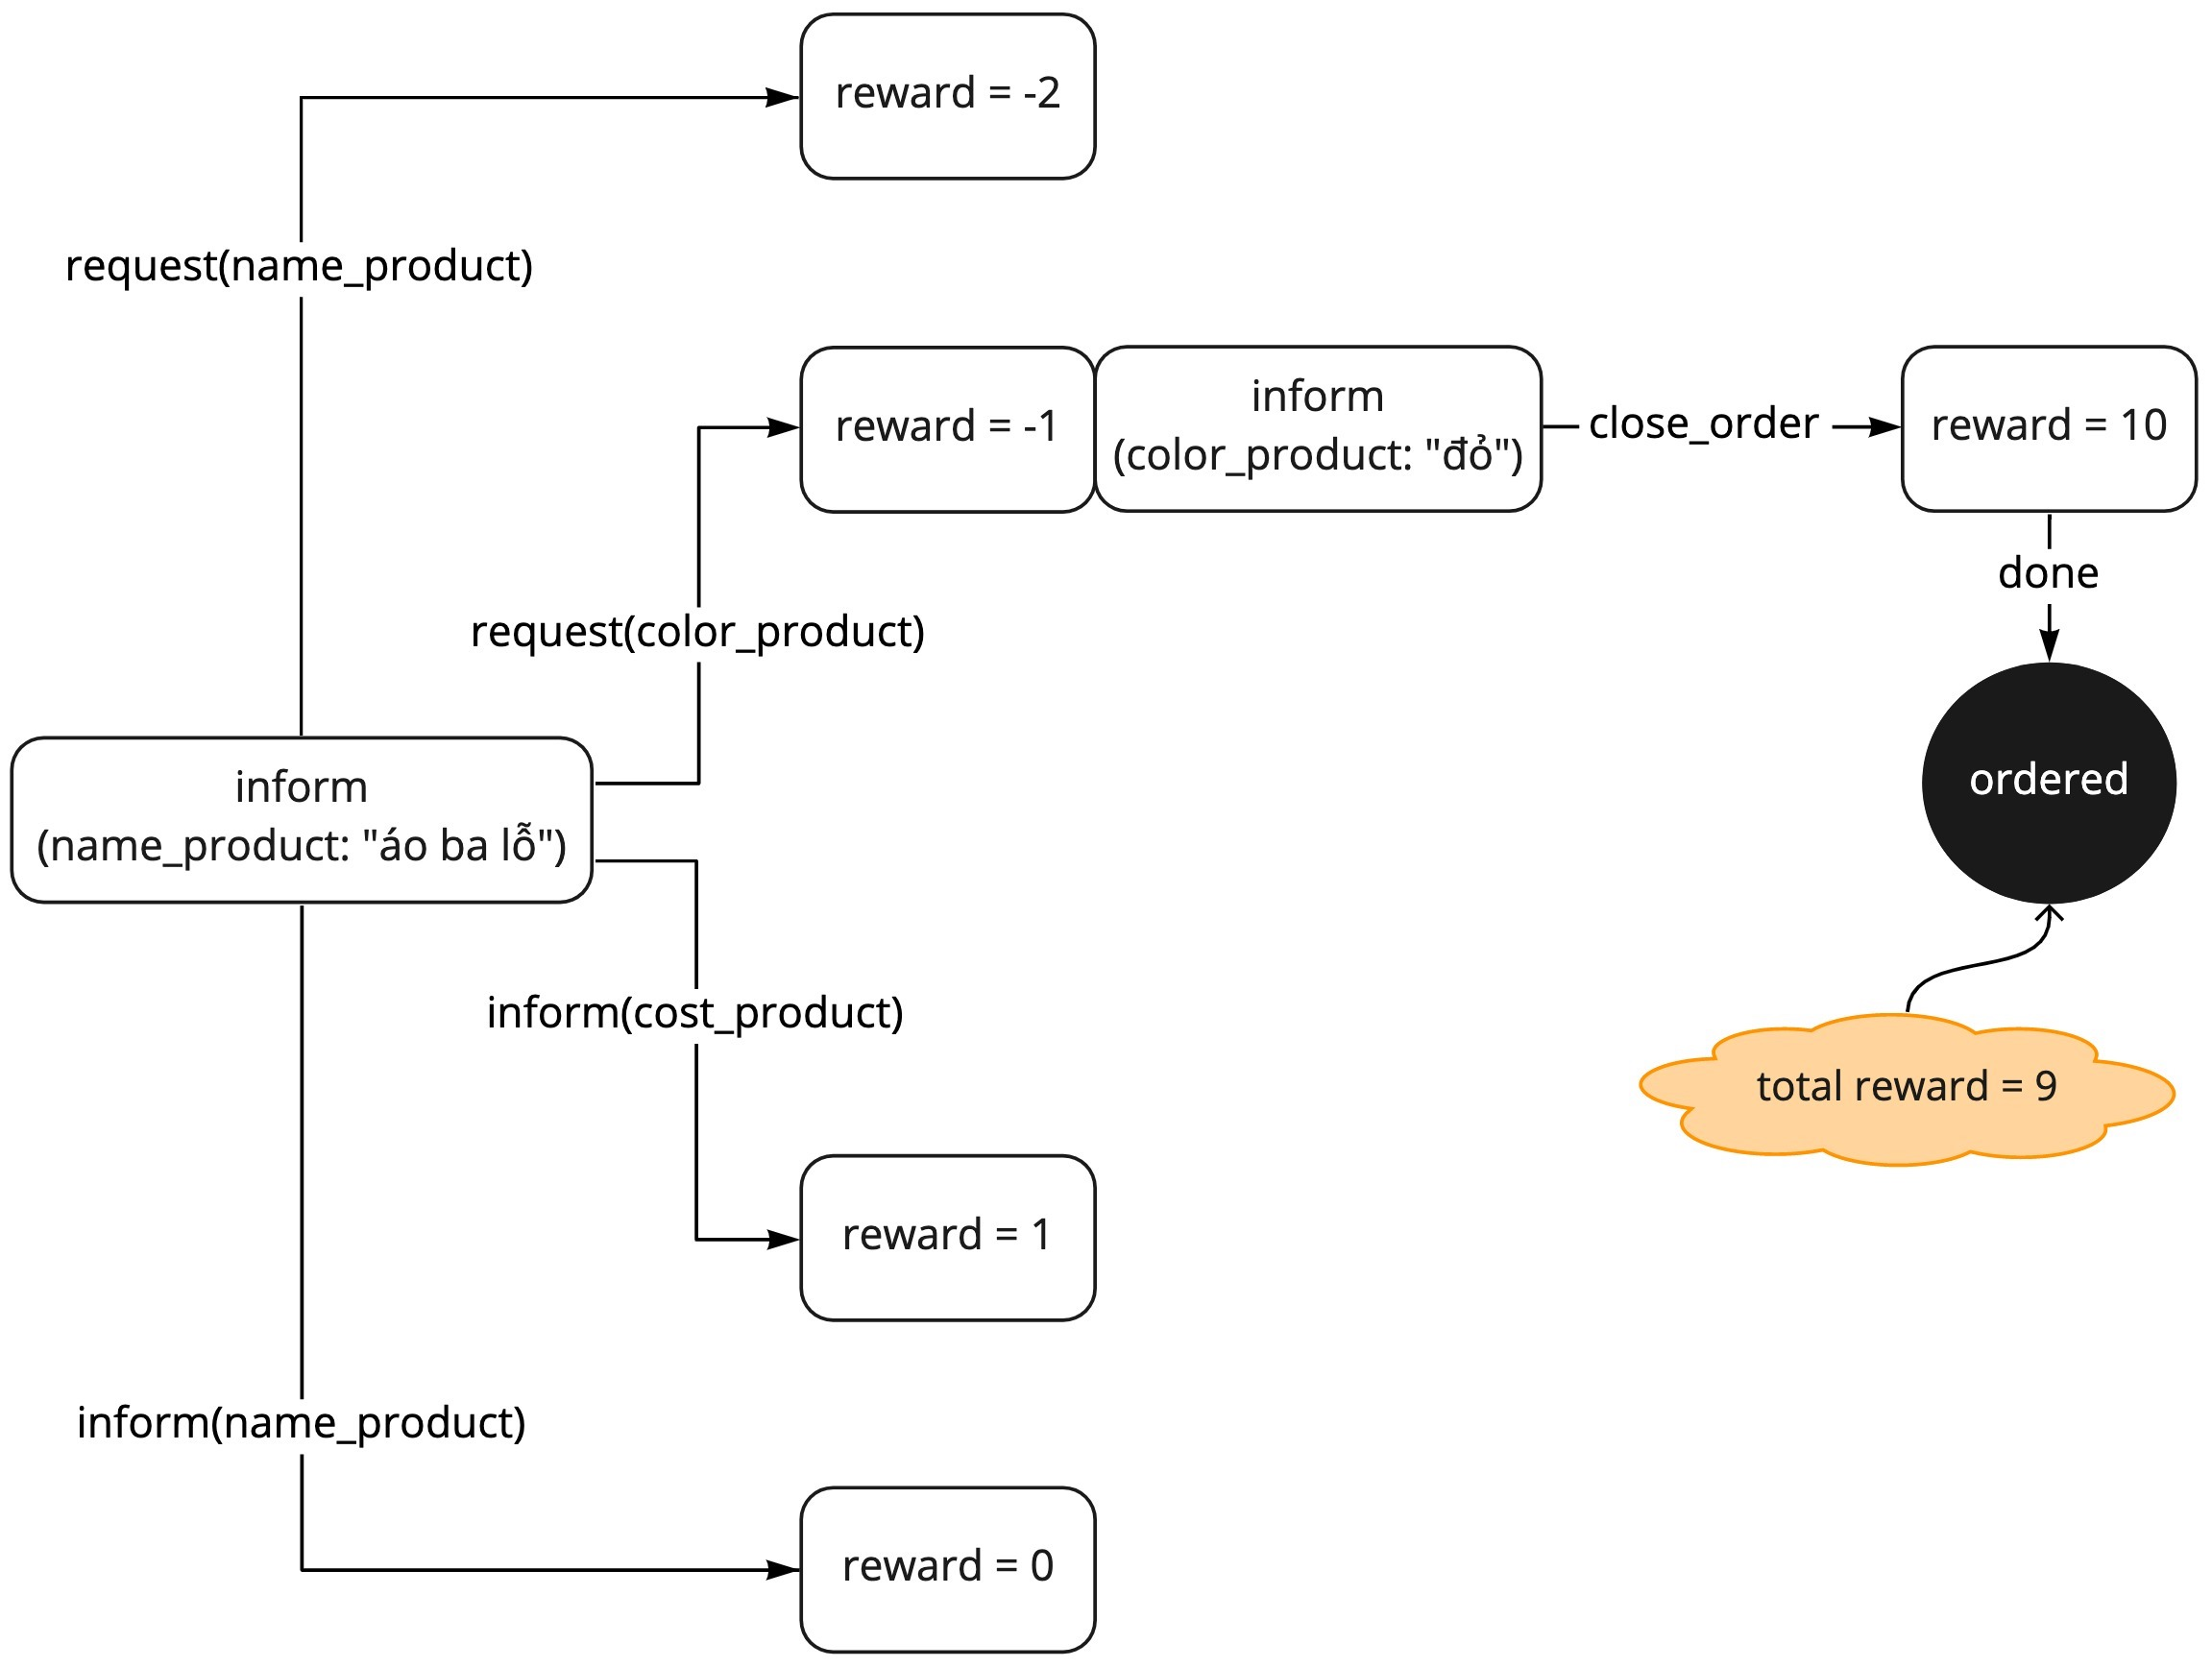
\includegraphics[scale=0.18]{chapter3/img/dialog_ex13.jpg}
        \end{center}
        \caption{Quá trình cho điểm thưởng và ra hành động - phương án 1}
        \label{fig:dialog2}
    \end{figure}
\end{center}

Ta có, quá trình một hội thoại với mục tiêu là chốt đơn hàng. Đầu tiên, người dùng cung cấp thông tin tên sản phẩm (áo ba lỗ). Và tác nhân có các hành động có thể có như sau:

\begin{itemize}
    \item Yêu cầu tên sản phẩm: người dùng đã cung cấp tên sản phẩm trước đó. Vì vậy, đây là hành vi không đúng, gây phiền nhiễu khó chịu cho người dùng. Nó nhận điểm trừ 2.
    \item Yêu cầu thông tin màu sắc: màu sắc là thông tin chưa được cung cấp, tuy nhiên đây là hành vi yêu cầu, không cung cấp thông tin hữu ích cho người dùng. Nó nhận điểm trừ 1.
    \item Thông báo giá sản phẩm: đây là hành vi cung cấp thông tin hữu ích. Nó nhận điểm thưởng 1.
    \item Thông báo tên sản phẩm: người dùng đã cung cấp tên sản phẩm trước đó. Vì vậy, đây là hành vi không cần thiết. Không nhận điểm thưởng nào.
\end{itemize}

Vì mục tiêu của hội thoại này là chốt đơn hàng. Và trong thực tế, ta cần biết đủ thông tin sản phẩm để có được một mẫu hàng duy nhất. Với sản phẩm này có nhiều màu, tác nhân cần yêu cầu người dùng cung cấp thông tin màu sắc sản phẩm mà họ muốn. Sau khi có được thông tin này, nó sẽ hoàn thành được mục tiêu hội thoại với hành động chốt đơn hàng và nhận được điểm thưởng 10. Với luồng hội thoại này, ta nhận được tổng phần thưởng là 9. Qua ví dụ này, ta thấy rằng để hoàn thành được mục tiêu cuối cùng của người dùng, ngoài việc xét điểm thưởng ở mỗi hành động, ta còn phải quan tâm đến phần thưởng của cả cuộc hội thoại.

Xét một trường hợp khác như hình \ref{fig:dialog3}.

\begin{center}
    \begin{figure}[h!]
        \begin{center}
         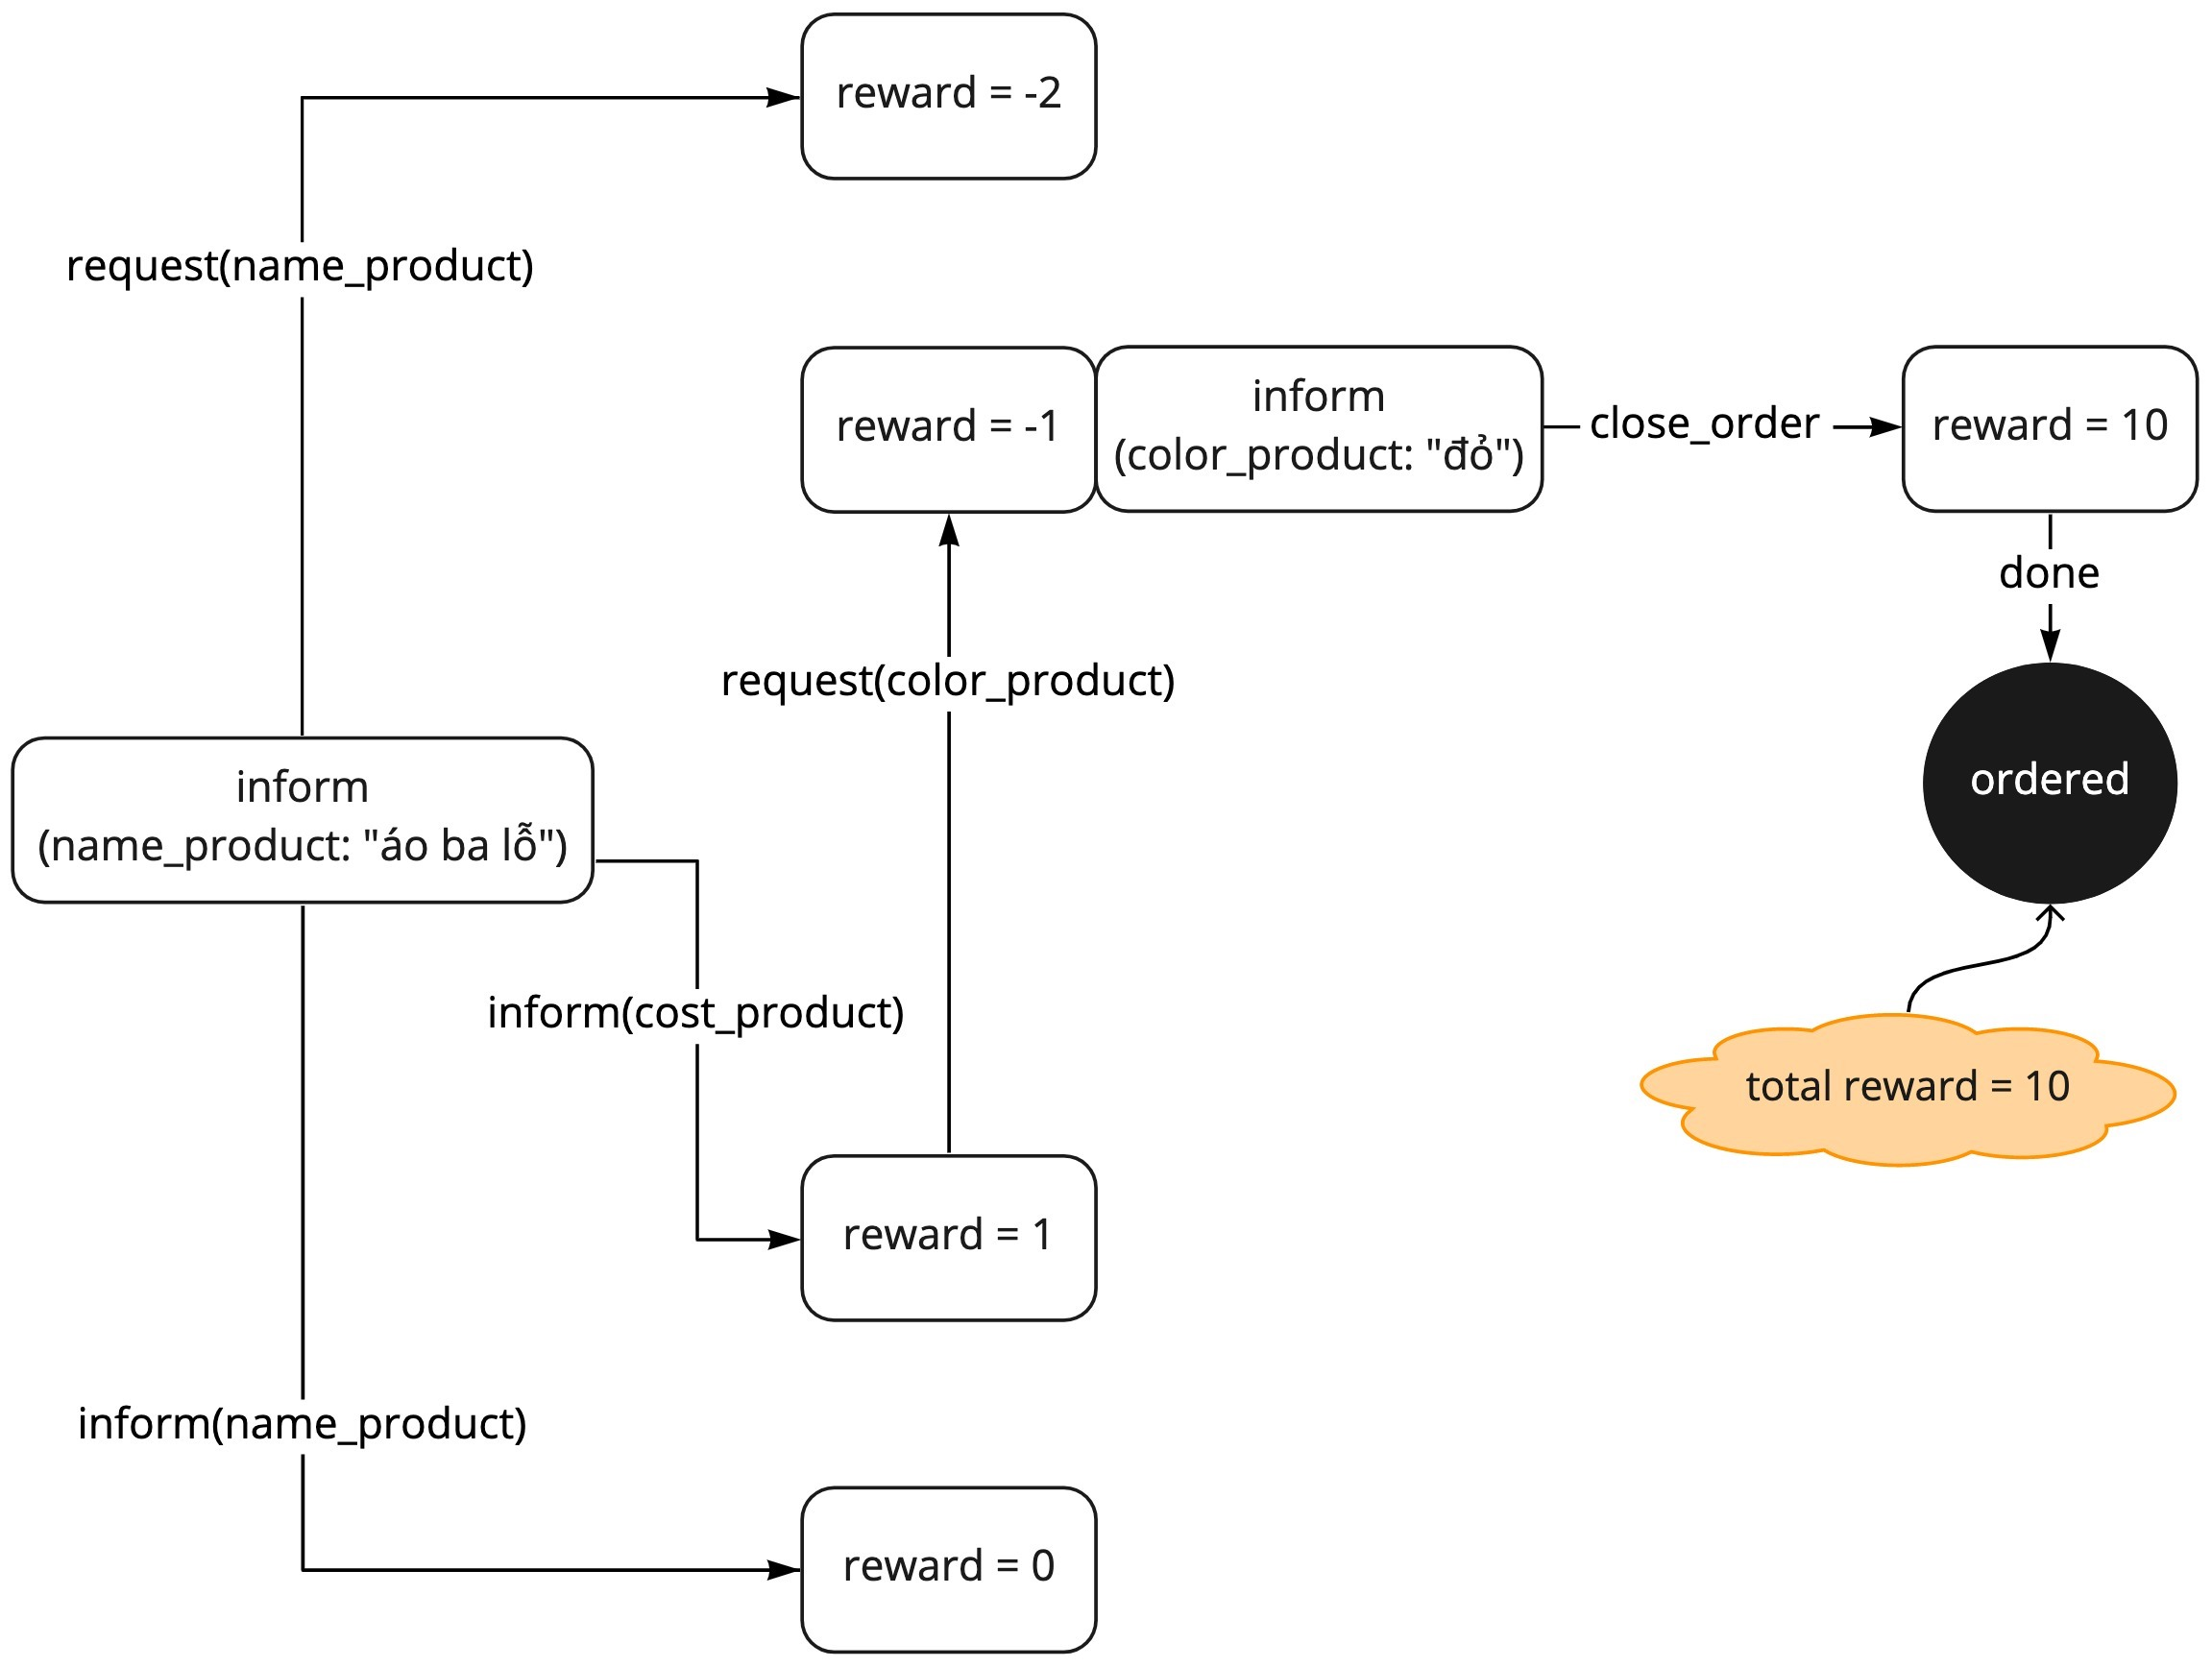
\includegraphics[scale=0.18]{chapter3/img/dialog_ex15.jpg}
        \end{center}
        \caption{Quá trình cho điểm thưởng và ra hành động - phương án 2}
        \label{fig:dialog3}
    \end{figure}
\end{center}

Thay vì ngay lập tức yêu cầu thông tin màu sắc, tác nhân có thể thông báo một thông tin hữu ích là giá đơn hàng, nhận được phần thưởng là 1. Mặc dù, nó không được yêu cầu bởi người dùng. Khi đó, tổng phần thưởng nhận được có giá trị là 10, cao hơn trường hợp lúc nãy. Tuy nhiên, như đã biết, ta mong đợi tác nhân hoàn thành mục tiêu cho người dùng nhanh nhất có thể. Hạn chế các hành động không cần thiết. Vì vậy, ngoài điểm thưởng cho từng hành động, quá trình tính tổng điểm thưởng, còn kèm theo một tham số, gọi là gamma ($\gamma$). Tham số này nhỏ hơn 1. Với mỗi điểm thưởng cho từng hành động sẽ được nhân với lũy thừa của gamma. Với bậc là số lượt hội thoại đã thực hiện cho đến hiện tại. Việc này sẽ làm giảm giá trị tổng điểm thưởng khi tác nhân càng đi nhiều bước (thực hiện nhiều hành động) trước khi đạt được mục tiêu cuối cùng. Cách tính tổng điểm thưởng như trên, ta gọi đó là tính giá trị Q (Q-value). Và cách học chọn hành động từ Q-value đó gọi là Q-Learning.

\subsection{Q-Learning}
Giả sử, tác nhân đang ở trạng thái $s$ và phải chọn một hành động $a$, nó sẽ nhận được phần thưởng $r$ và đạt trạng thái mới $s'$. Cách mà tác nhân chọn được gọi là \textit{policy}.

\begin{equation*}
    s \xrightarrow{\text{a}} r,s'
\end{equation*}

Ta định nghĩa một hàm $Q(s,a)$ sao cho khi nhận vào trạng thái $s$ và hành động $a$ nó sẽ trả về một giá trị ước lượng là tổng phần thưởng mà ta sẽ đạt được tại trạng thái đó khi ta thực hiện hành động $a$ và thực hiện một số \textit{policy} tiếp theo sau đó. Ta chắc chắn rằng sẽ luôn có các \textit{policy} tối ưu, nghĩa là nó luôn chọn được hành động tốt nhất. Ta gọi hàm $Q$ trong trường hợp luôn có \textit{policy} tối ưu là $Q^*$. Nếu ta biết được hàm $Q^*$, ta chỉ cần áp dụng chiến lược tham lam (greedy) lên hàm đó. Cụ thể với mỗi trạng thái $s$, ta sẽ chọn một hành động $a$ sao cho cực đại hoá hàm $Q^*$, hay ${max_a}{Q^*}(s,a)$. Mục tiêu của chúng ta là tìm được hàm đủ tốt để ước lượng được hàm $Q^*$ rồi sau đó áp dụng chiến lược tham lam lên nó. Ta viết lại hàm $Q^*$ ở dạng sau:

\begin{equation*}
    Q^*(s,a) = r_0 + {\gamma}r_1 + {\gamma}^{2}r_2 + {\gamma}^{3}r_3 + ...
\end{equation*}

Hàm $Q^*$ lúc này là tổng giá trị của phần thưởng nhận được sau mỗi hành động tính từ hành động $a$ trở đi. $\gamma$ là giá trị khấu hao của phần thưởng sau mỗi hành động và nó luôn nhỏ hơn 1 để đảm bảo rằng công thức này có giới hạn. Vì có hệ số mũ nên giá trị phần thưởng sẽ giảm dần và tiến về 0. Hệ số $\gamma$ vì vậy mà sẽ điều khiển mức độ phụ thuộc vào tương lai của hàm $Q$ tại trạng thái $s$.\newline

Ta có thể viết lại hàm $Q^*$ ở trên như sau:

\begin{equation*}
    Q^*(s,a) = r_0 + {\gamma}(r_1 + {\gamma}r_2 + {\gamma}^{2}r_3 + ...) = r_0 + {\gamma}max_{a}Q^{*}(s',a)
\end{equation*}

Công thức này cho thấy giá trị hàm $Q$ của hành động $a$ tại trạng thái $s$ bằng phần thưởng $r(s,a)$ cộng với giá trị hàm $Q$ lớn nhất của các trạng thái $s'$ tiếp theo khi thực hiện các hành động $a$. Do đó, với công thức này chúng ta có thể tạo ra một ma trận trạng thái-hành động (state-action) như một bảng tìm kiếm (lookup table). Từ đó với mỗi trạng thái, tác nhân chỉ cần tìm hành động nào có giá trị hàm $Q$ lớn nhất là xong.\newline

Tuy nhiên, trong thực tế số lượng trạng thái rất lớn và ta không thể nào lưu trữ toàn bộ chúng như cách ở trên được. Vì vậy ta sẽ xấp xỉ hàm $Q$ bằng một mạng nơ-ron. Mạng nơ-ron này sẽ nhận đầu vào là một trạng thái và nó sẽ ước lượng giá trị của hàm $Q$ cho mỗi một hành động. Và khi ta sử dụng nhiều tầng, ta được mạng nơ-ron học sâu.

\subsection{Deep Q-Learning}
\label{subsec:deepqlearning}
Q-Learning hoạt động tốt khi chúng ta có một môi trường tương đối đơn giản để giải quyết, nhưng khi số lượng trạng thái và hành động chúng ta có thể thực hiện trở nên phức tạp hơn, chúng ta sử dụng mạng nơ-ron học sâu như một công cụ xấp xỉ hàm.

Trạng thái được đưa ra làm đầu vào và giá trị Q của tất cả các hành động của tác nhân có thể có làm đầu ra. Sự so sánh giữa Q-learning và Deep Q-Learning được minh họa như hình \ref{fig:dqlearning} \cite{introductiondeepqlearningpython}.

\begin{center}
    \begin{figure}[h!]
        \begin{center}
         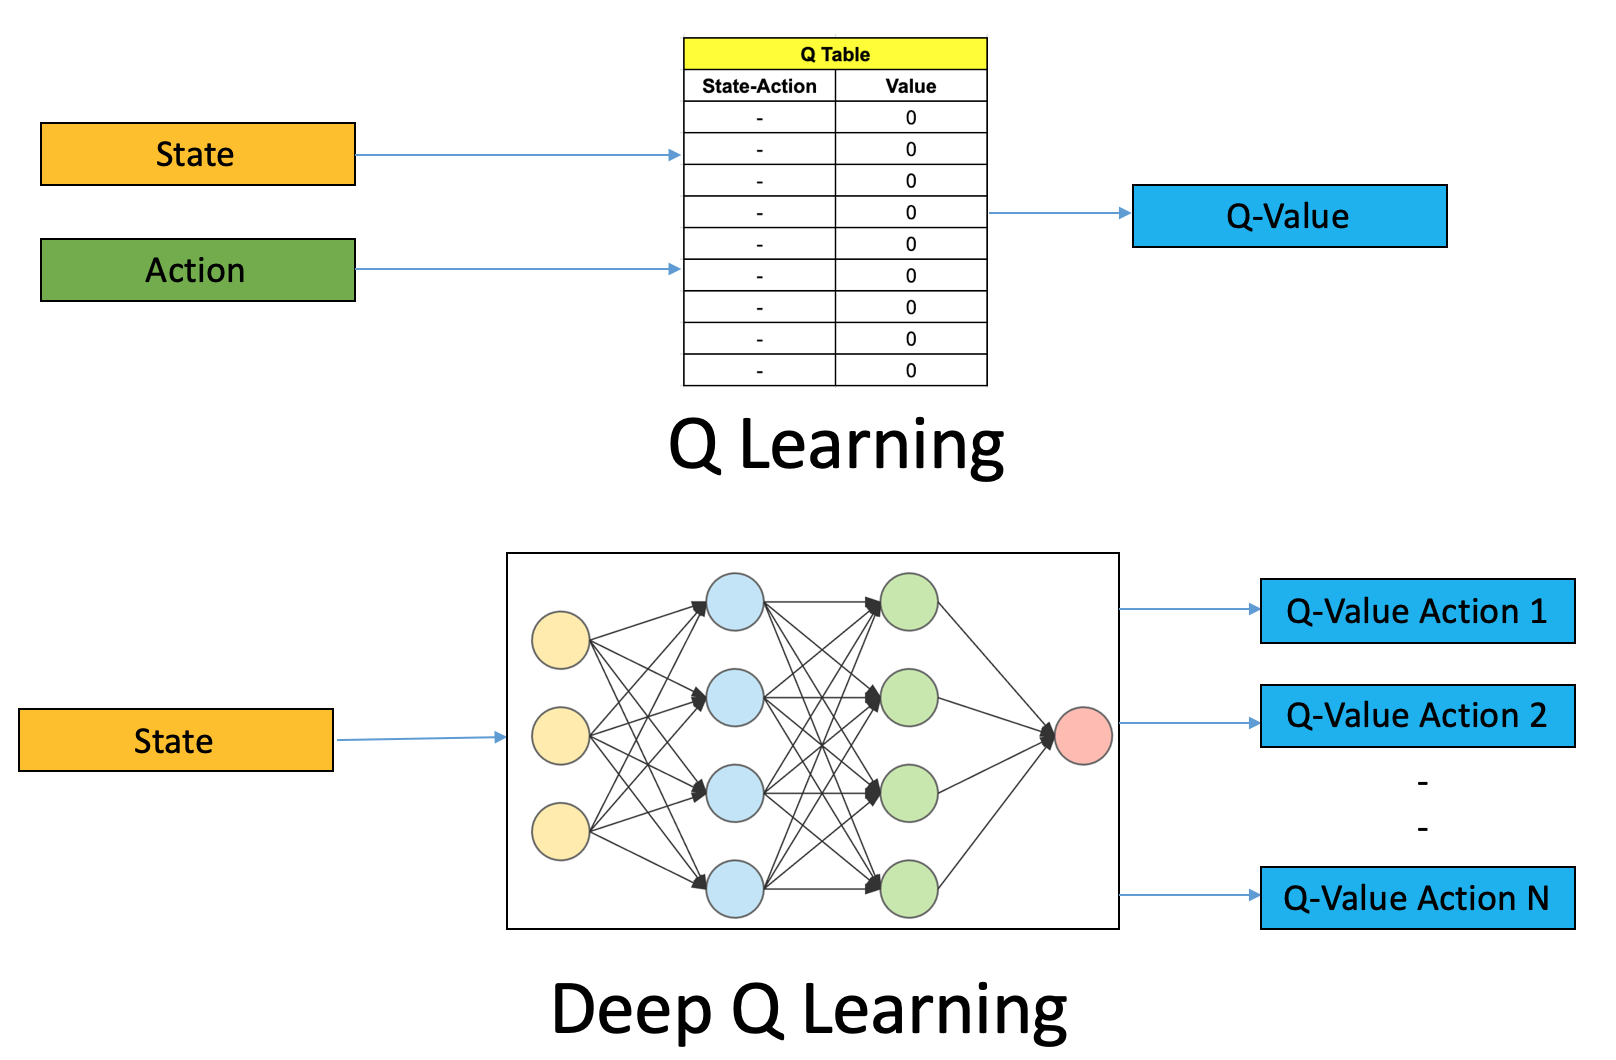
\includegraphics[scale=0.27]{chapter3/img/dqlearning.png}
        \end{center}
        \caption{Q-Learning và Deep Q-Learning}
        \label{fig:dqlearning}
    \end{figure}
\end{center}

Ta xét ví dụ sau, để làm rõ cách cập nhật trọng số của mạng nơ-ron và chọn ra hành động.

Giả sử, trạng thái hội thoại được rút gọn lại thành chỉ chứa các ý định hành động hiện tại của người dùng lần lượt là: hello, inform, request, reject, done. Ta mã hóa về dạng one-hot vec-tơ để làm đầu vào cho mạng nơ-ron. Các hành động có thể có của tác nhân là: hello, match\_found, request, done. Mạng nơ-ron huấn luyện trong ví dụ này như hình \ref{fig:examnetwork}. Activation của tầng ẩn là ReLU, tầng đầu ra là linear.

\begin{center}
    \begin{figure}[h!]
        \begin{center}
         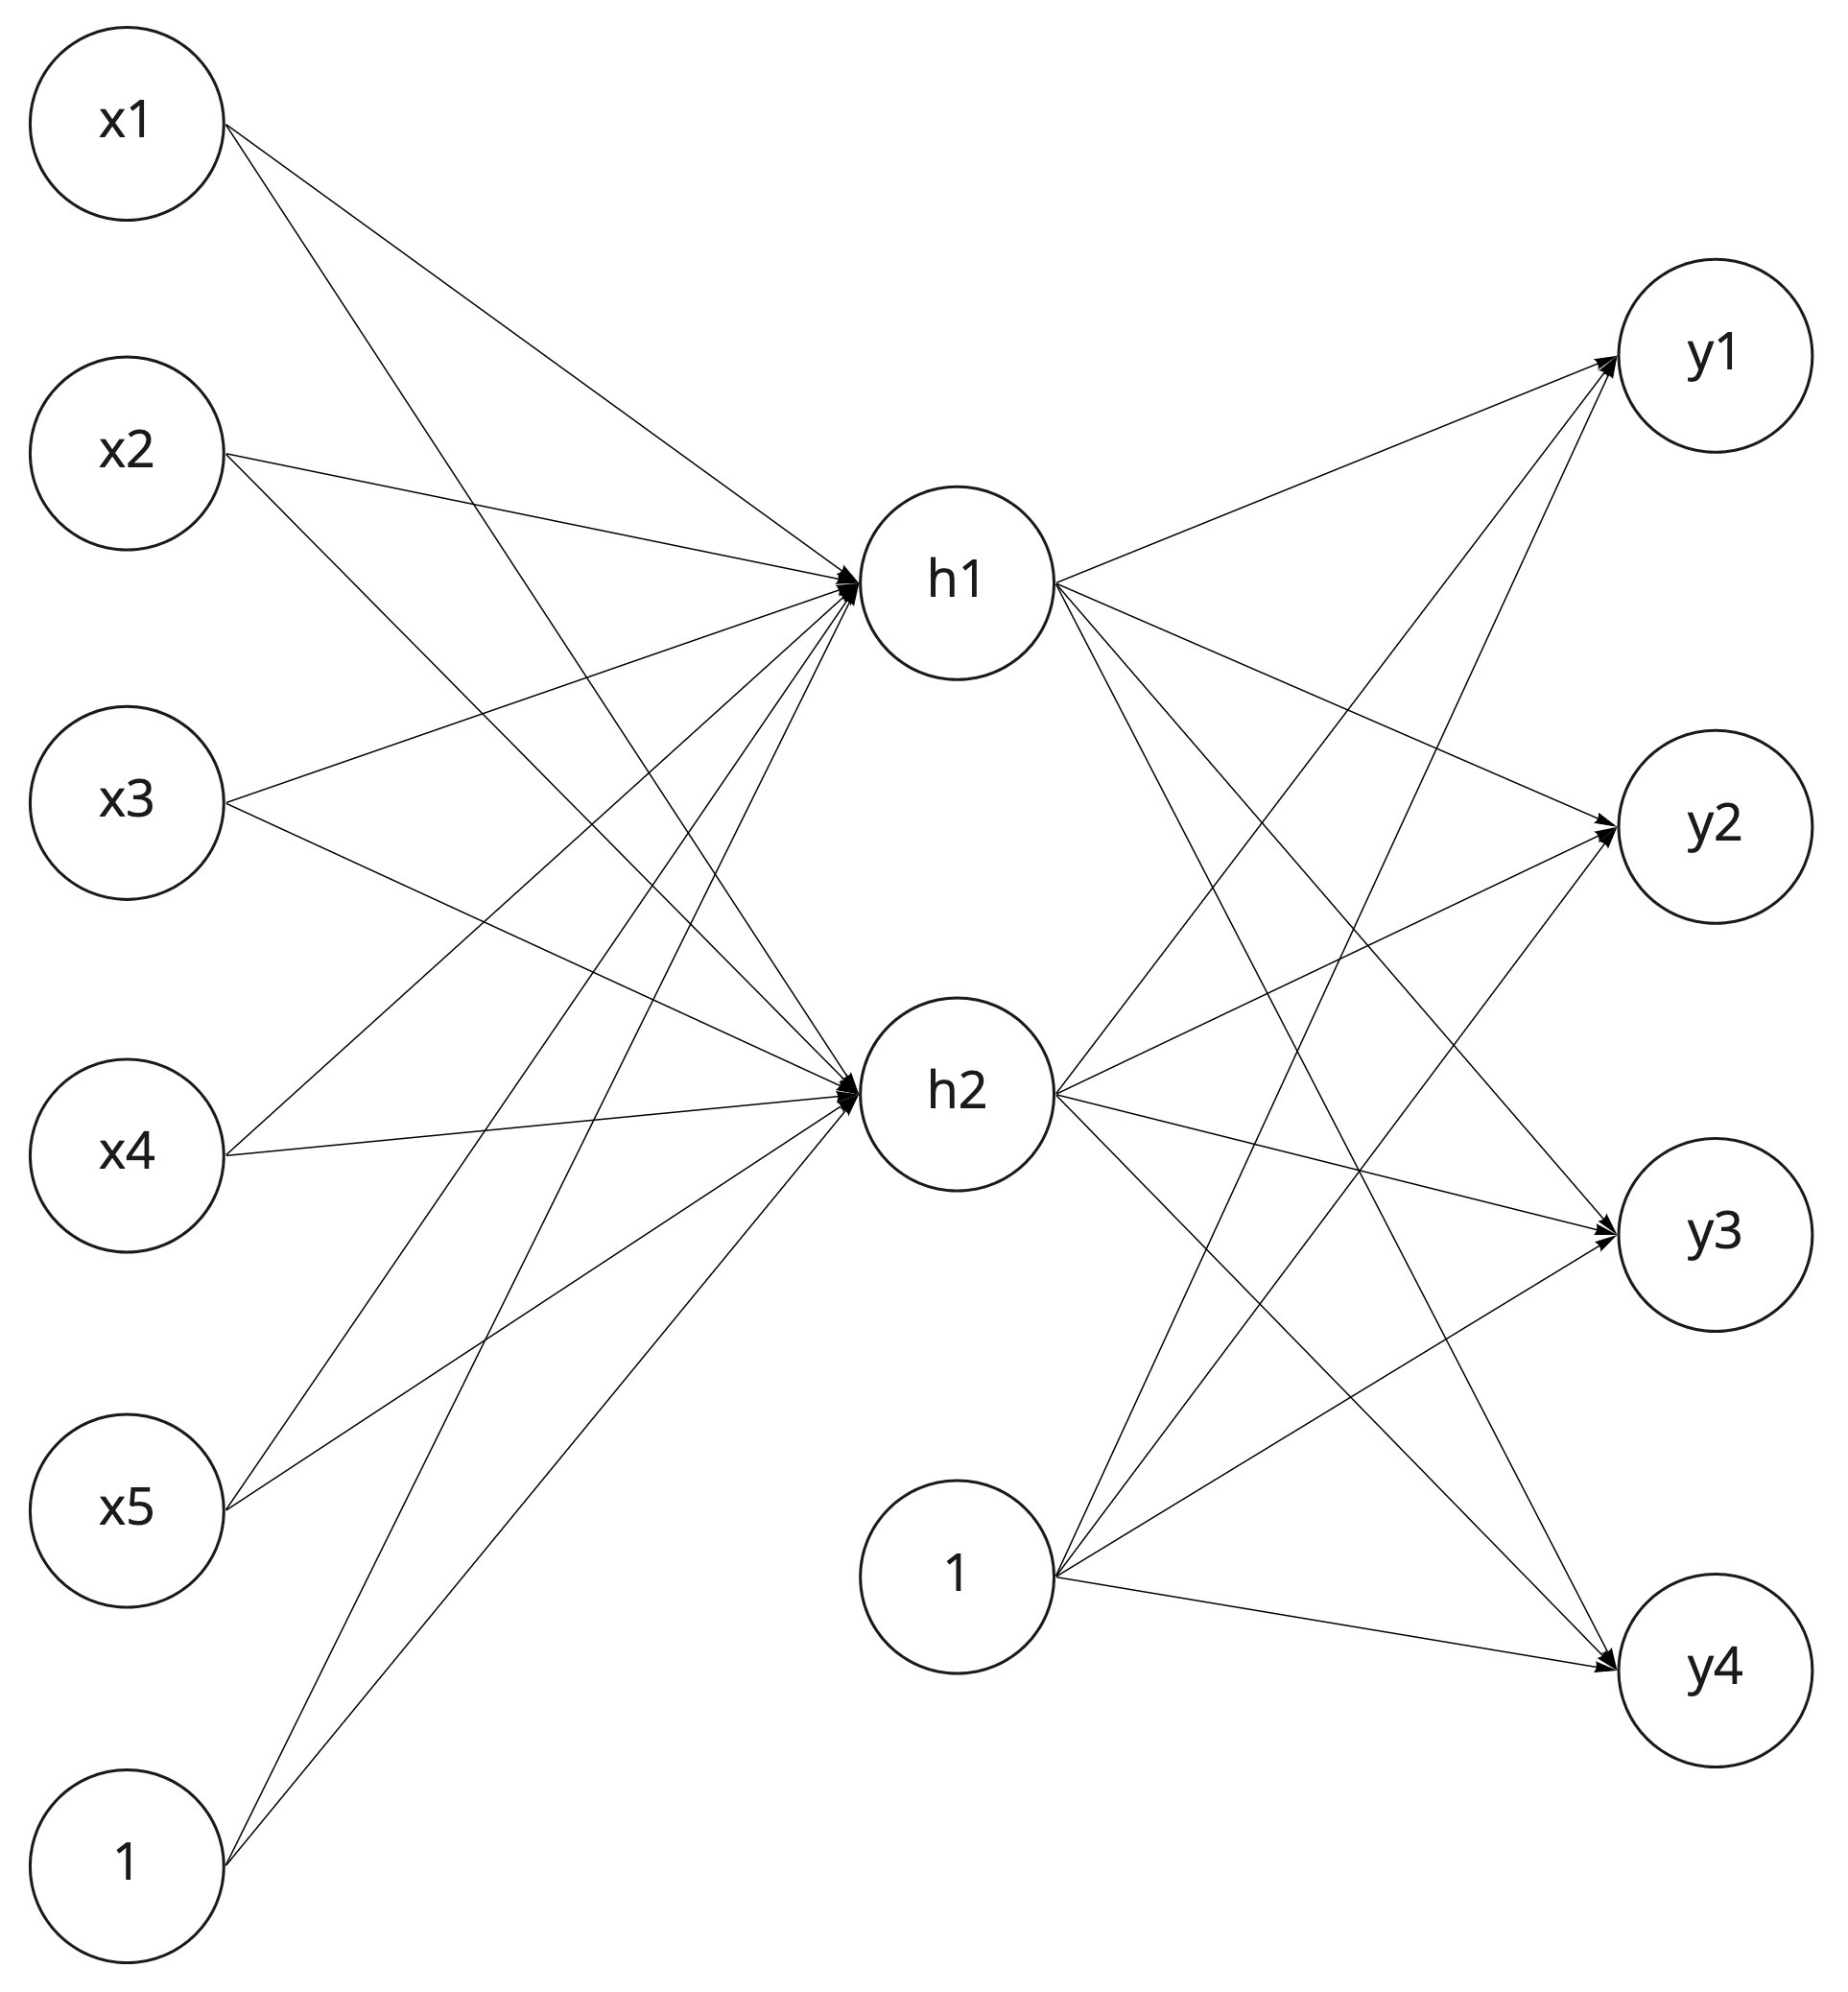
\includegraphics[scale=0.15]{chapter3/img/neural_network.jpg}
        \end{center}
        \caption{Mạng nơ-ron học sâu Q-Learing}
        \label{fig:examnetwork}
    \end{figure}
\end{center}

Giả sử, ta có ma trận trọng số cho mạng nơ-ron này như sau:

\begin{equation*}
    w_1 = 
    \begin{bmatrix}
        0.18998 & 0.871522 & 0.31542 & 0.691079 & 0.902874 \\
        0.12114 & 0.84606 & 0.902874 & 0.09224 & 0.19652302
    \end{bmatrix}
\end{equation*}

\begin{equation*}
    w_2 = 
    \begin{bmatrix}
        0.52141 & 0.63489 \\
        0.130012 & 0.12001 \\
        0.113114 & 0.12121 \\
        0.53514 & 0.62465
    \end{bmatrix}
\end{equation*}

\begin{equation*}
    bias = 0.325
\end{equation*}

\renewcommand{\lstlistingname}{Ví dụ}
\begin{lstlisting}[caption={Một mẫu đoạn hội thoại},label={exam:dialog3},language=exam_en,firstnumber=1]
User: hello
Agent: hello
User: request
Agent: match_found
User: done
\end{lstlisting}

Sử dụng đoạn hội thoại mẫu \ref{exam:dialog3} để huấn luyện. Ta có hành động đầu tiên của người dùng là hello. Trạng thái đầu vào $s$ như sau:

\begin{equation*}
    s = 
    \begin{bmatrix}
        1 \\
        0 \\
        0 \\
        0 \\
        0
    \end{bmatrix}
\end{equation*}

Sau khi cho qua mạng nơ-ron, ta có kết quả lần lượt là:

\begin{equation*}
    w_1*s + bias = 
    \begin{bmatrix}
        0.51498 \\
        0.44614
    \end{bmatrix}
\end{equation*}

\begin{equation*}
    h = relu(w_1*s + bias) = 
    \begin{bmatrix}
        0.51498 \\
        0.44614
    \end{bmatrix}
\end{equation*}

\begin{equation*}
    y = h*w_2 + bias = 
    \begin{bmatrix}
        0.876765546 \\
        0.445494841 \\
        0.437328077 \\
        0.879267748
    \end{bmatrix}
\end{equation*}

Kết quả ma trận y là giá trị Q cho từng hành động của tác nhân theo thứ tự là hello, match\_found, request, done. Với kết quả trên, ta thấy Q-value của hành động done là lớn nhất. Dễ thấy rằng, với hành động này, không hoàn thành được mục tiêu toàn cục. Vì vậy, ta cần cập nhật Q-value của hành động tốt nhất tại thời điểm này.

Vì done là hành vi kết thúc hội thoại, mà hiện tại nó chưa hoàn thành mục tiêu người dùng, nên nhận điểm trừ rất lớn là $r_0 = -10$. Nhìn lại công thức tính $Q^*$ mục tiêu. Giả sử $\gamma = 0.9$

\begin{equation*}
    Q^*(s,a) = r_0 + {\gamma}max_{a}Q^{*}(s',a)
\end{equation*}

Để có $Q(s',a)$, ta cho đầu vào mạng nơ-ron là trạng thái kế tiếp $s'$. Dựa vào mẫu hội thoại huấn luyện trên, ta có trạng thái đầu vào $s'$ như sau:

\begin{equation*}
    s' = 
    \begin{bmatrix}
        0 \\
        0 \\
        1 \\
        0 \\
        0
    \end{bmatrix}
\end{equation*}

Sau khi cho qua mạng nơ-ron, ta nhận được kết quả đầu ra là:

\begin{equation*}
    y = 
    \begin{bmatrix}
        1.438486316 \\
        0.555619444 \\
        0.546271075 \\
        1.434705853
    \end{bmatrix}
\end{equation*}

Ta có $Q$ lớn nhất với trạng thái đầu vào $s'$ là 1.438486316.

\begin{equation*}
    => Q^*(s,a) = -10 + 0.9*1.438486316 = -8.705362316
\end{equation*}

Sau đó, mô hình sẽ được huấn luyện lại với đầu vào là trạng thái $s$ và giá trị $Q$ được cập nhật lại như sau:

\begin{equation*}
    y = 
    \begin{bmatrix}
        0.876765546 \\
        0.445494841 \\
        0.437328077 \\
        -8.705362316
    \end{bmatrix}
\end{equation*}
